%%%%%%%%%%%%%%%%%%%%%%%%%%%%%%%%%%%%%%%%%%%%%%%%%%%%%%%%%%%%%%%%%%%%%

\documentclass[paper=a4,fontsize=11pt]{temp} % KOMA-article class
\usepackage[english]{babel}
\usepackage{hyperref}
% pers date
\def\mydate{\leavevmode\hbox{\the\year-\twodigits\month-\twodigits\day}}
\def\twodigits#1{\ifnum#1<10 0\fi\the#1}

% per header/footer

\usepackage{fancyhdr}
\pagestyle{fancy}
\renewcommand{\headrulewidth}{0pt}
\renewcommand{\footrulewidth}{0.4pt}
\fancyhead[C]{}
\cfoot{
    In accordo con il Decreto Legislativo n. 196 datato 30/06/2003, Autorizzo all'uso e al processamento dei miei dati personali contenuti in questo documento.
    Versione aggiornata al \mydate. 
    \newline
    \thepage
}

\usepackage{lipsum}% provides filler text


%%%%%%%%%%%%%%%%%%%%%%%%%%%%%%%%%%%%%%%%%%%%%%%%%%%%%%%%%%%%%%%%%%%%%%%%%%%%%%
\begin{document}

% Upload a your photo and rename it to "photo.png" or "photo.jpg"
\begin{minipage}{.2\linewidth}
   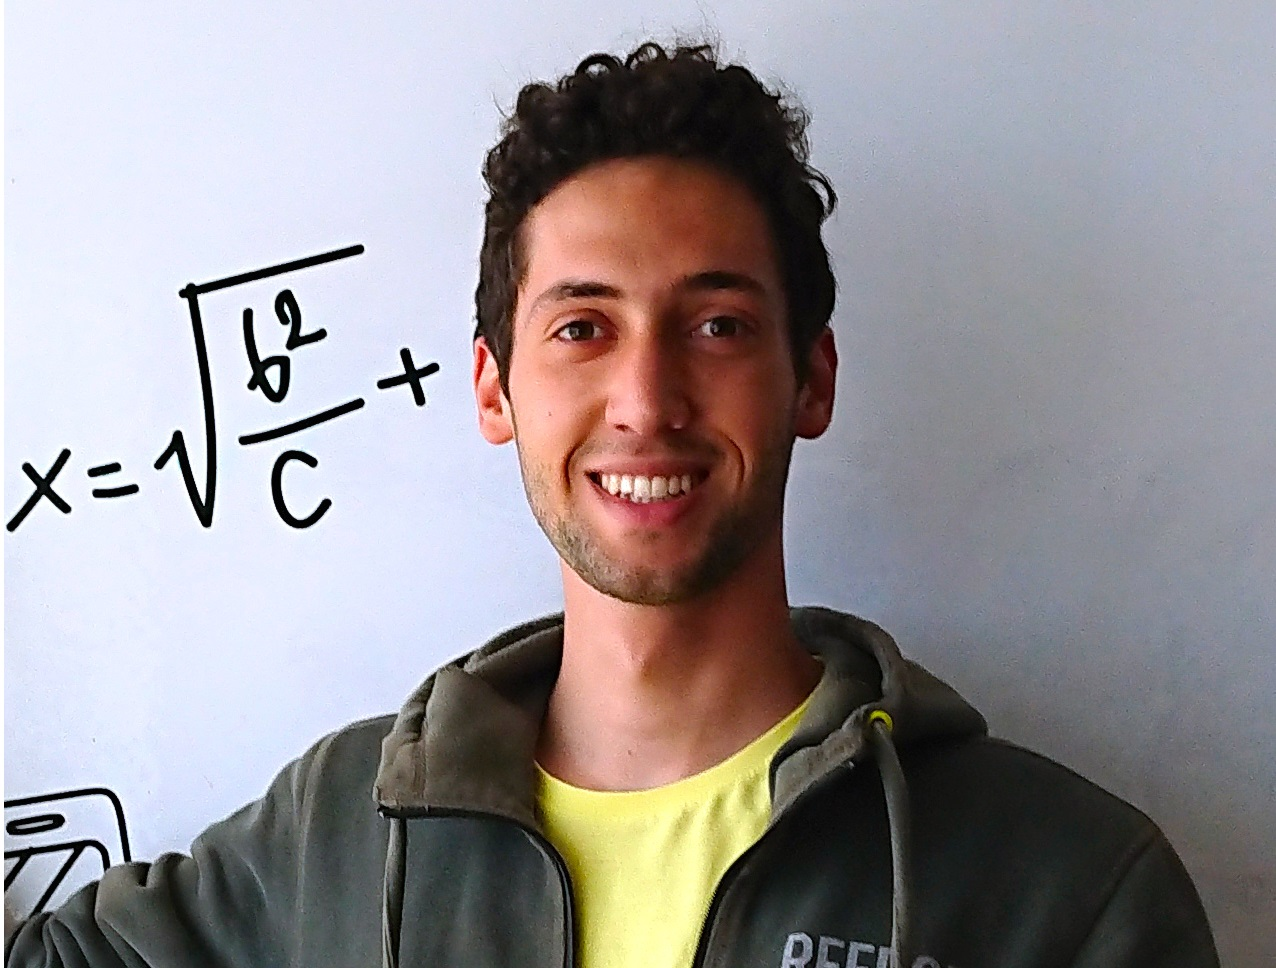
\includegraphics[width=1\textwidth]{photo}
\end{minipage}      
\begin{minipage}{0.7\linewidth}
    \MyName{Igor Lirussi}
    \sepspace
    \noindent
    % info 
    \hfill Genere: M | Nazionalità: Italiana | Stato Civile: Single | Nascita: 25/12/1995

    \hfill igor.lirussi@studio.unibo.it | +39 3317055048 
    
    \hfill GitHub/LinkedIn: igor-lirussi | Skype: igor.lirussi
    
    \hfill via VI Maggio, 24, 33030, Forgaria nel Friuli (UD), Italy
 

\end{minipage}


%%%%%%%%%%%%%%%%%%%%%%%%%%%%%%%%%%%%%%%%%%%%%%%%%%%%%%%%%%%%%%%%%%%%%%%%%%%%%%%%
\NewPart{Esperienza Lavorativa}{}

\noindent

\shortEntry{RESEARCH ASSISTANT - ROBOTICA}{Apr 2020 - Sep 2020}
{Stoccolma (SE) \href{https://www.kth.se/is/rpl}{KTH Royal Institute of Technology: Robotic Perception and Learning Department}}
{
 \begin{itemize}
    \item Human Robot Interaction
    \item Dialog Engines
 \end{itemize}
} {IMG/kth}

\sepspace

\shortEntry{RESEARCH SCHOLAR - COMPUTER VISION}{Sep 2018 - Sep 2019 }
{Lisbona (PT) \href{https://welcome.isr.tecnico.ulisboa.pt/}{ I.S.R. Institute for Systems and Robotics - VisLab}}
{
 \begin{itemize}
    \item Object recognition and Dialog Processing for Human Robot Interaction
    \item SLAM and Visual Navigation Systems
 \end{itemize}
} {IMG/ist}

%%%%%%%%%%%%%%%%%%%%%%%%%%%%%%%%%%%%%%%%%%%%%%%%%%%%%%%%%%%%%%%%%%%%%%%%%%%%%%%%
\NewPart{EDUCAZIONE}{}
\noindent

\longEntry{\href{https://corsi.unibo.it/2cycle/ComputerScienceEngineering}{MAGISTRALE INGEGNERIA E SCIENZE INFORMATICHE}}
{Set 2019 - oggi}
{Università di Bologna}
{Distributed Systems, Machine Learning,    Languages, Compilers and Computational Models,    Information Systems,     Concurrent and Distributed Programming,    Programming and Development paradigms,    Web Services and Applications,     Smart City and Mobile Technologies,     Agile, Continuous Integration and Delivery,  } 
 {IMG/unibo}

\sepspace

\longEntry{\href{https://dsv.su.se/en/}{ERASMUS Magistrale}}
{Gen 2020 - Lug 2020}
{Università di Stoccolma}
{Decision Making and Business Intelligence, Network Security, Cyber Forensics}
{IMG/stockholmuni}

\sepspace

\longEntry{\href{https://ciencias.ulisboa.pt/en}{ERASMUS Triennale}}
{Set 2018 - Set 2019}
{Università di Lisbona}
{Artificial Intelligence, Operational Research} 
{IMG/ulisboa}

\sepspace

\longEntry{\href{https://corsi.unibo.it/1cycle/ComputerScienceEngineering}{TRIENNALE INGEGNERIA E SCIENZE INFORMATICHE}}
{Set 2014 - Set 2019}
{Università di Bologna}
{Software Engineering, Embedded Systems and IoT, Automatic Controls, Mobile Application Programming, Operating Systems, Object-Oriented Programming, Network Programming, Telecommunications Networks, Law for Information Technology, Fundamentals of Image Processing, Databases, Algorithms and Data Structures, Computer Architecture, C Programming} 
{IMG/unibo}


%%%%%%%%%%%%%%%%%%%%%%%%%%%%%%%%%%%%%%%%%%%%%%%%%%%%%%%%%%%%%%%%%%%%%%%%%%%%%%%%
\NewPart{Lingue e Interessi}{}
\hspace{3mm}
\begin{minipage}[t]{0.30\textwidth} 
\begin{tabular}[t]{ l l }
\flag{IMG/flag/it}  & Madrelingua \\
\flag{IMG/flag/gb}  & Proficienza Professionale \\
\flag{IMG/flag/pt}  & Livello conversazionale \\
\flag{IMG/flag/se}  & Livello base \\
\end{tabular}
\end{minipage}
%
\begin{minipage}[t]{0.66\textwidth} 
\begin{tabular}[t]{l l}
Corso per aziende teorico e pratico di primo soccorso.\\

Corso di cinema con regista Alessandro Quadretti.\\
Cuoco e sportivo\\
Volontario al Banco Alimentare.\\
Donatore di Sangue.\\
%\software{IMG/soft/writeL}  	 & Latex Writing\\
%\software{IMG/soft/office} 		 & This software experience. fillertext fillertext fillertex\\
%\software{IMG/soft/Matlab}  	 & This software experience. fillertext fillertext fillertex\\
%\software{IMG/soft/office} 		 & This software experience. fillertext fillertext fillertex\\
%\software{IMG/soft/Matlab}  	 & This software experience. fillertext fillertext fillertex\\
\end{tabular}
\end{minipage}


%%% References

\end{document}
